%*********************************************************************
\subsection{Simulation Experiment}\label{sub:bc_simulation_experiment}
%*********************************************************************

% Introductory paragraph

% The statistical calibration framework revisited

% Observation Layout

% Modeling the simulator output

% Modeling the discrepancy

% Likelihood Formulation

% Full Probability Model
% Different Model
% 1. TC, DP, and CO only
% 2. All Output, Discrepancy
% 3. All Output, No Discrepancy
% 4. 

% Analyzing convergence

\clearpage
\begin{sidewaysfigure}
	\centering
	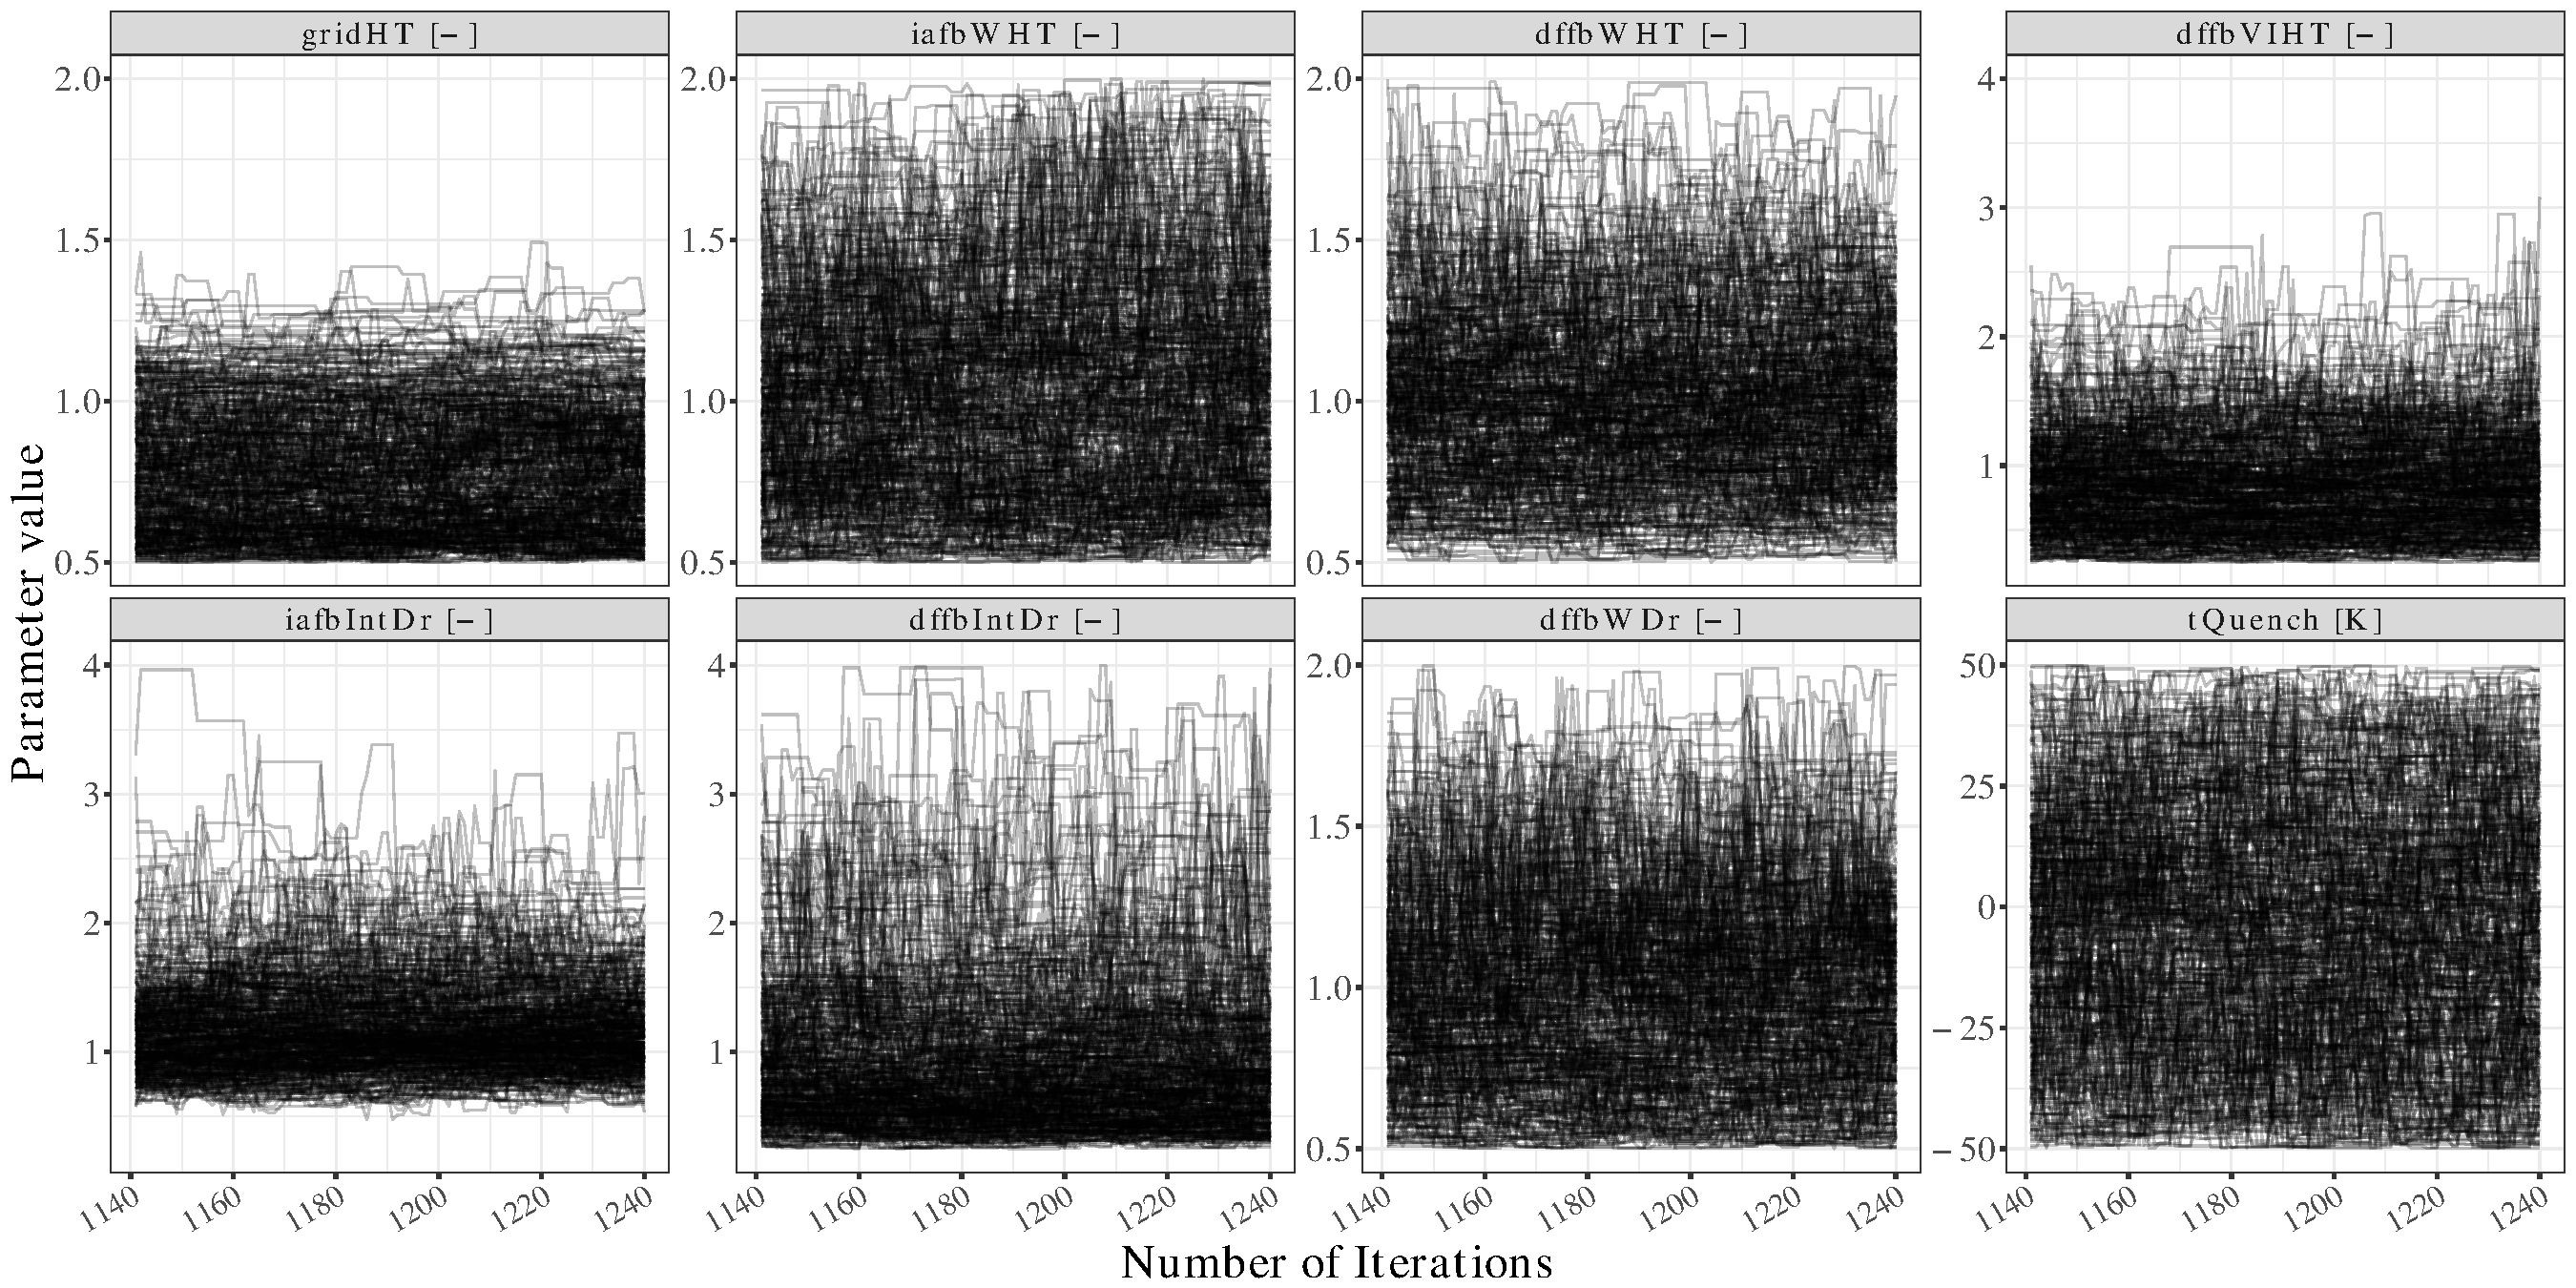
\includegraphics[width=0.90\textwidth]{../figures/chapter5/figures/plotEnsTraceDiscAllCentered}
		\captionof{figure}[Ensemble trace plots for each model parameter of calibration with model bias term.]{Ensemble trace plots for each model parameter of calibration with model bias term. Shown here is for the last $100$ iterations (out of $1'240$ post-burn-in iterations) and for $400$ walkers (out of $1'000$ walkers).}
	\label{fig:ch5_plot_ens_trace_all_disc_centered}
\end{sidewaysfigure}
\clearpage